\begin{frame}{Marco teórico - Estados cuánticos}
\begin{defi}
Un bit cuántico, qbit o qubit es la unidad básica de información cuántica, es la
versión cuántica del clásico bit binario.
\end{defi}
\center{Estados basicos del qubit.}
\begin{minipage}{0.4\linewidth}
\begin{equation*}
\left| 0\right\rangle    
\end{equation*}
\end{minipage}
\begin{minipage}{0.4\linewidth}
\begin{equation*}
\left| 1\right\rangle    
\end{equation*}
\end{minipage}
Por convención se llega a utilizar la siguiente expresión:
\begin{equation*}
\left| 1100\right\rangle    \rightarrow \left|12 \right\rangle
\end{equation*}
\end{frame}

\begin{frame}{Marco teórico - Compuertas lógicas clásicas y cuánticas - Compuerta NOT}
\vspace{0.5cm}
 \begin{minipage}{0.49\linewidth}
    \begin{figure}[H]
        \centering
        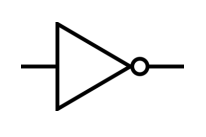
\includegraphics[height=2.5cm]{images/not.png}
        \caption{Representación gráfica de la compuerta NOT.}
    \end{figure}
    \begin{table}[H]
        \centering
        \begin{tabular}{cc} \hline
            A & NOT(A)\\ \hline
            0 & 1 \\
            1 & 0 \\ \hline
        \end{tabular}
        \caption{Compuerta clásica NOT.}
    \end{table}
\end{minipage}
\begin{minipage}{0.49\linewidth}
    \begin{figure}[H]
        \centering
        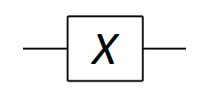
\includegraphics[height=2.1cm]{images/not_c.png}
        \caption{Representación gráfica de la compuerta cuántica NOT.}
    \end{figure}
    \begin{table}[H]
        \centering
        \begin{tabular}{cc} \hline
            A & NOT(A) \\ \hline
            $\left| 0 \right\rangle$ & $\left| 1 \right\rangle$ \\
            $\left| 1\right\rangle$ & $\left| 0 \right\rangle$ \\
            $\left| \psi \right\rangle$ & $\hat{X}\left| \psi \right\rangle$ \\ \hline
        \end{tabular}
        \caption{Compuerta cuántica NOT.}
    \end{table}
\end{minipage} 
\end{frame}
\begin{frame}{Compuertas lógicas clásicas y cuánticas - Compuerta de Hadamard}
\begin{minipage}{0.49\linewidth}
   \begin{equation*}
    \left| 0 \right\rangle \underset{\hat{H}}{\rightarrow} \frac{\left| 0 \right\rangle+\left| 1\right\rangle }{\sqrt{2}} \equiv \left| + \right\rangle
    \end{equation*}
    \begin{equation*}
      \left| 1 \right\rangle \underset{\hat{H}}{\rightarrow} \frac{\left| 0 \right\rangle-\left| 1\right\rangle }{\sqrt{2}} \equiv \left| - \right\rangle  
    \end{equation*}
    \center{donde:}
    \begin{equation*}
        \hat{H} = \frac{1}{\sqrt{2}} \left(\begin{matrix}
            1 & 1 \\
            1 & -1
        \end{matrix} \right)
    \end{equation*}
\end{minipage} 
\begin{minipage}{0.49\linewidth}
    \begin{figure}[H]
        \centering
        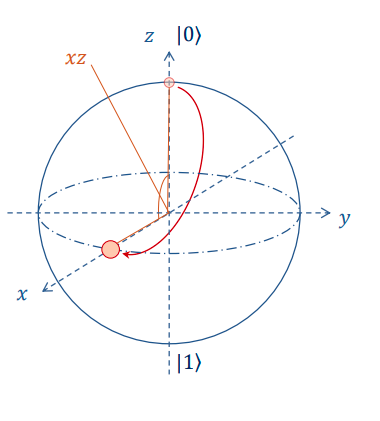
\includegraphics[scale=0.3]{images/hadamard.png}
        \caption{Representación gráfica del efecto de la transformación de Hadamard aplicada a un qubit.} 
    \end{figure}
\end{minipage} 
\end{frame}
\begin{frame}{Compuertas lógicas clásicas y cuánticas - Compuerta de desplazamiento de fase}
    \begin{equation*}
    \left| 0 \right\rangle \underset{\hat{R}(\phi)}{\rightarrow} \left| 0 \right\rangle
    \end{equation*}
    \begin{equation*}
    \left| 1\right\rangle \underset{\hat{R}(\phi)}{\rightarrow} e^{i\phi}\left| 1\right\rangle
    \end{equation*}
    \center{donde:}
    \begin{equation*}
        \hat{R}(\phi) = \left[\begin{matrix}
            1 & 0 \\
            0 & e^{i\phi}
        \end{matrix} \right]
    \end{equation*}
\end{frame}
\begin{frame}{Compuertas lógicas clásicas y cuánticas - Compuerta SWAP}
\begin{minipage}{0.49\linewidth}
\begin{equation*}
    U_{SWAP}=\left[\begin{matrix}
    1 & 0 & 0 & 0\\
    0 & 0 & 1 & 0\\
    0 & 1 & 0 & 0\\
    0 & 0 & 0 & 1\\
    \end{matrix}\right]
\end{equation*}
\end{minipage}
\begin{minipage}{0.49\linewidth}
\begin{figure}[H]
        \centering
        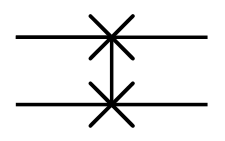
\includegraphics[scale=0.7]{images/swap_gate.png}
        \caption{Representación gráfica de la compuerta SWAP.}
    \end{figure}
\end{minipage}
\end{frame}
\begin{frame}{Compuertas lógicas clásicas y cuánticas - Compuerta Controlada}
\begin{minipage}{0.49\linewidth}
\begin{equation*}
    U_{CNOT}=\left[\begin{matrix}
    1 & 0 & 0 & 0\\
    0 & 1 & 0 & 0\\
    0 & 0 & 0 & 1\\
    0 & 0 & 1 & 0\\
    \end{matrix}\right]
\end{equation*}
\end{minipage}
\begin{minipage}{0.49\linewidth}
\begin{figure}[H]
        \centering
        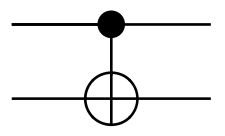
\includegraphics[scale=0.7]{images/not_gate.png}
        \caption{Representación gráfica de la compuerta NOT controlada.}
    \end{figure}
\end{minipage}
\end{frame}
\begin{frame}{Transformada de Fourier Cuántica}
 \begin{equation*}
    \left|\tilde{x} \right\rangle \equiv QFT\left| x \right\rangle= \frac{1}{\sqrt{N}} \sum\limits_{y=0}^{N-1} e^{\frac{2\pi i x y}{N}} \left|y \right\rangle
\end{equation*} 
\begin{equation*}
    \left|\tilde{x} \right\rangle =\frac{1}{\sqrt{N}} \bigotimes\limits_{k=1}^N \left[\left|0 \right\rangle+e^{2\pi i x 2^{-k}} \left| 1\right\rangle  \right].
\end{equation*}
\end{frame}
\begin{frame}{Transformada de Fourier Cuántica}
    \begin{figure}[H]
    \begin{subfigure}{0.49\linewidth}
        \centering
        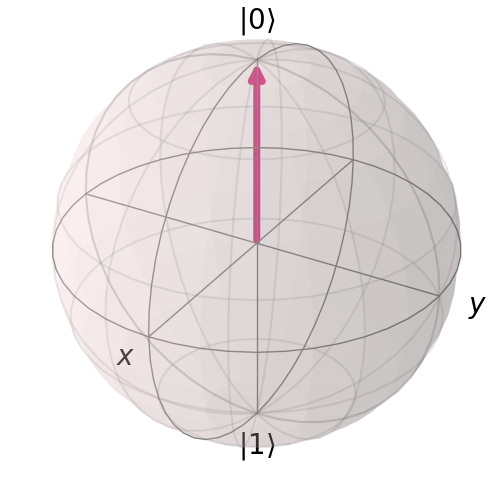
\includegraphics[scale=0.125]{images/0.png}
        \caption{Qubit con el estado cuántico $\left|0 \right\rangle$ representado en la esfera de Bloch.}
    \end{subfigure}
    \begin{subfigure}{0.49\linewidth}
        \centering
        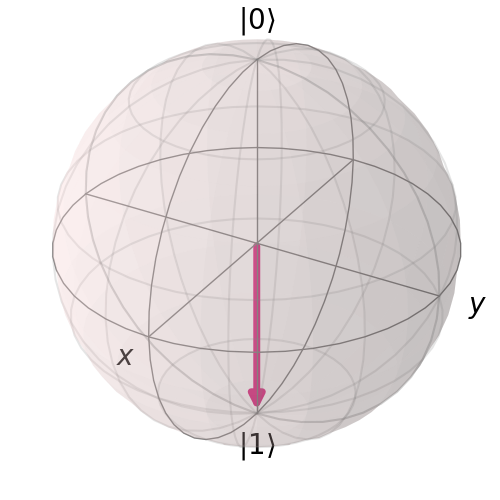
\includegraphics[scale=0.125]{images/1.png}
        \caption{Qubit con el estado cuántico $\left|1 \right\rangle$ representado en la esfera de Bloch.}
    \end{subfigure}
    \begin{subfigure}{0.49\linewidth}
        \centering
        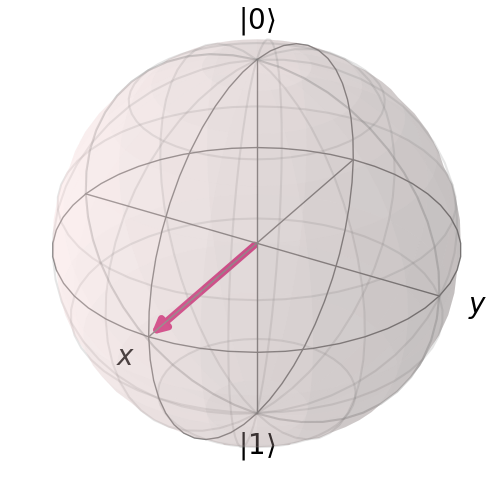
\includegraphics[scale=0.125]{images/2.png}
        \caption{Qubit con el estado cuántico $\left|\tilde{0} \right\rangle$ representado en la esfera de Bloch.}
    \end{subfigure}
    \begin{subfigure}{0.49\linewidth}
        \centering
        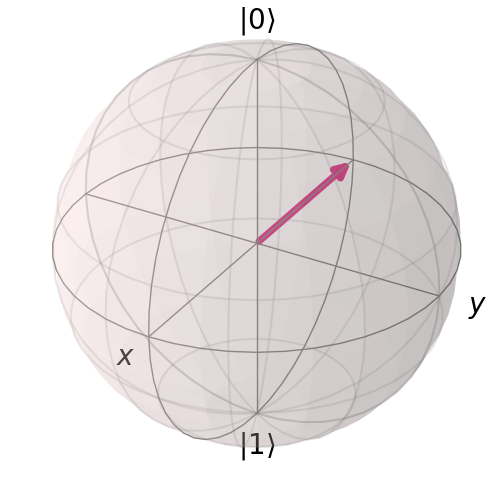
\includegraphics[scale=0.125]{images/3.png}
        \caption{Qubit con el estado cuántico $\left|\tilde{1} \right\rangle$ representado en la esfera de Bloch.}
    \end{subfigure}
\caption{Representación en la esfera de Bloch de los estados bases computacionales cuánticos y las bases de Fourier.}
\label{fig:QFT_bloch}
\end{figure}
\end{frame}
\begin{frame}{Estimación de Fase Cuántica (QPE)}
    \begin{equation*}
    \mathcal{U} \left|\psi \right\rangle = e^{i\theta_\psi}\left|\psi \right\rangle.
\end{equation*}
\end{frame}
\begin{frame}{Periodo de la función a\textsuperscript{x}mod N}
    \begin{equation}
        f(x)=a^xmod N
        \label{eq:axmodn}
        \end{equation}
    \begin{equation}
        a^rmodN=1
        \label{eq:condicionr}
    \end{equation}
Usando como ejemplo a=3 y N=35, se tiene el siguiente periodo:
\begin{figure}[H]
    \centering
    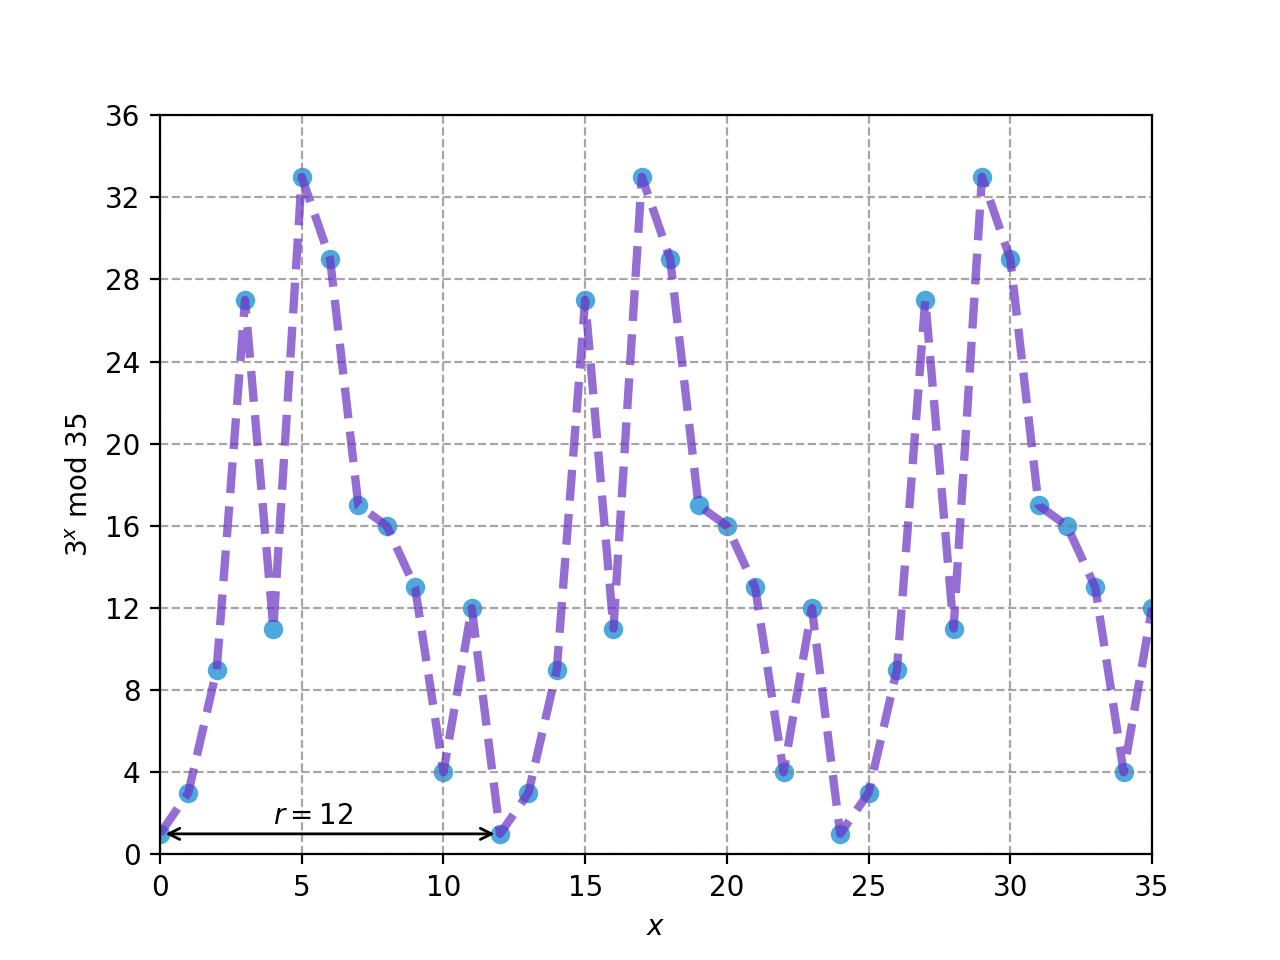
\includegraphics[scale=0.35]{images/period.png}
    \caption{Periodo de la función \ref{eq:axmodn} para visualizar la condición \ref{eq:condicionr}}
    \label{fig:condicionr}
\end{figure}
\end{frame}
\begin{frame}{Periodo de la función a\textsuperscript{x}mod N}
    \begin{minipage}{0.49\linewidth}
    \begin{align*}
    \mathcal{U}\left| 1 \right\rangle &= \left|3\right\rangle \\
    \mathcal{U}^2\left| 1 \right\rangle &= \left|9\right\rangle \\
    \mathcal{U}^3\left| 1 \right\rangle &= \left|12\right\rangle \\ 
                   & \vdots  \\ 
    \mathcal{U}^{r-1}\left| 1 \right\rangle &= \left|12\right\rangle \\
    \mathcal{U}^r\left| 1 \right\rangle &= \left|1\right\rangle \\
\end{align*}
    \end{minipage}
    \begin{minipage}{0.49\linewidth}
    \begin{equation}
    \left| u_0 \right\rangle = \frac{1}{\sqrt{r}} \sum\limits_{k=0}^{r-1} \left|a^k mod N \right\rangle.
    \label{eq:u0}
\end{equation}
    \end{minipage}
\end{frame}
\begin{frame}{Periodo de la función a\textsuperscript{x}mod N}
    \begin{align*}
    \left| u_0 \right\rangle &= \frac{1}{\sqrt{12}} \left(\left|1\right\rangle + \left|3\right\rangle+ \left|9\right\rangle 
    +\cdots +\left|4\right\rangle + \left|12\right\rangle \right)\\
    U\left| u_0 \right\rangle &= \frac{1}{\sqrt{12}} \left(U\left|1\right\rangle + U\left|3\right\rangle+ U\left|9\right\rangle 
    +\cdots +U\left|4\right\rangle + U\left|12\right\rangle \right)\\
    &= \frac{1}{\sqrt{12}} \left(\left|3\right\rangle + \left|9\right\rangle+ \left|27\right\rangle 
    +\cdots +\left|12\right\rangle + \left|1\right\rangle \right)\\
    &= \left| u_0 \right\rangle .
\end{align*}
\end{frame}
\begin{frame}{Periodo de la función a\textsuperscript{x}mod N}
\begin{align*}
    \left| u_1 \right\rangle &= \frac{1}{\sqrt{r}} \sum\limits_{k=0}^{r-1} e^{-\frac{2\pi i k}{r}} \left| a^k mod N \right\rangle \\
    U\left| u_1 \right\rangle &= e^{\frac{2\pi i}{r}} \left| u_1 \right\rangle.
\end{align*}
\begin{equation*}
    \frac{1}{\sqrt{r}} \sum\limits_{s=0}^{r-1} \left|u_s \right\rangle =  \left| 1 \right\rangle.
\end{equation*}
\end{frame}
\begin{frame}{Periodo de la función a\textsuperscript{x}mod N}
\vspace{1cm}
    \begin{figure}[H]
    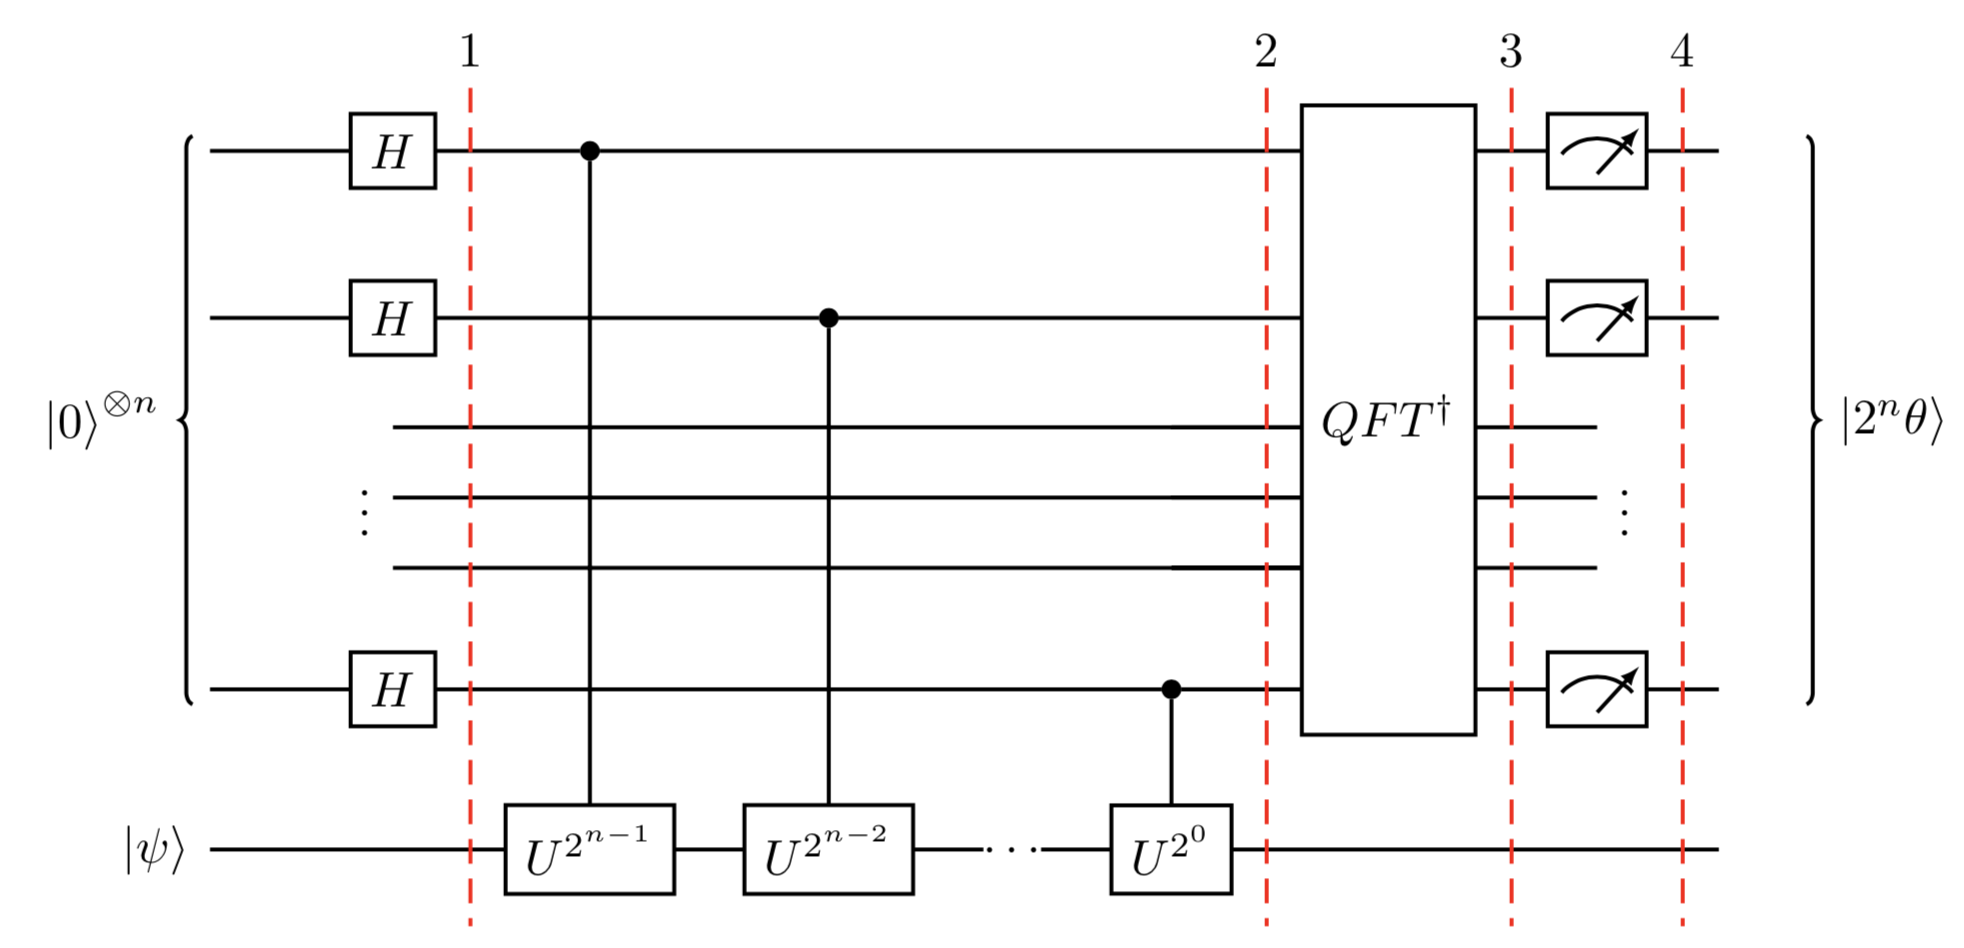
\includegraphics[scale=0.3]{images/qpe.png}
    \caption{Circuito cuántico que realiza el algortimo QPE (Quantum Phase Estimation) sobre una serie de qubits.}
    \label{fig:qpe}
\end{figure}
\end{frame}